\documentclass[tikz,border=8pt]{standalone}
\usepackage[T1]{fontenc}
\usepackage{lmodern}
\usepackage{tikz}
\usetikzlibrary{arrows.meta,positioning,calc}

\begin{document}
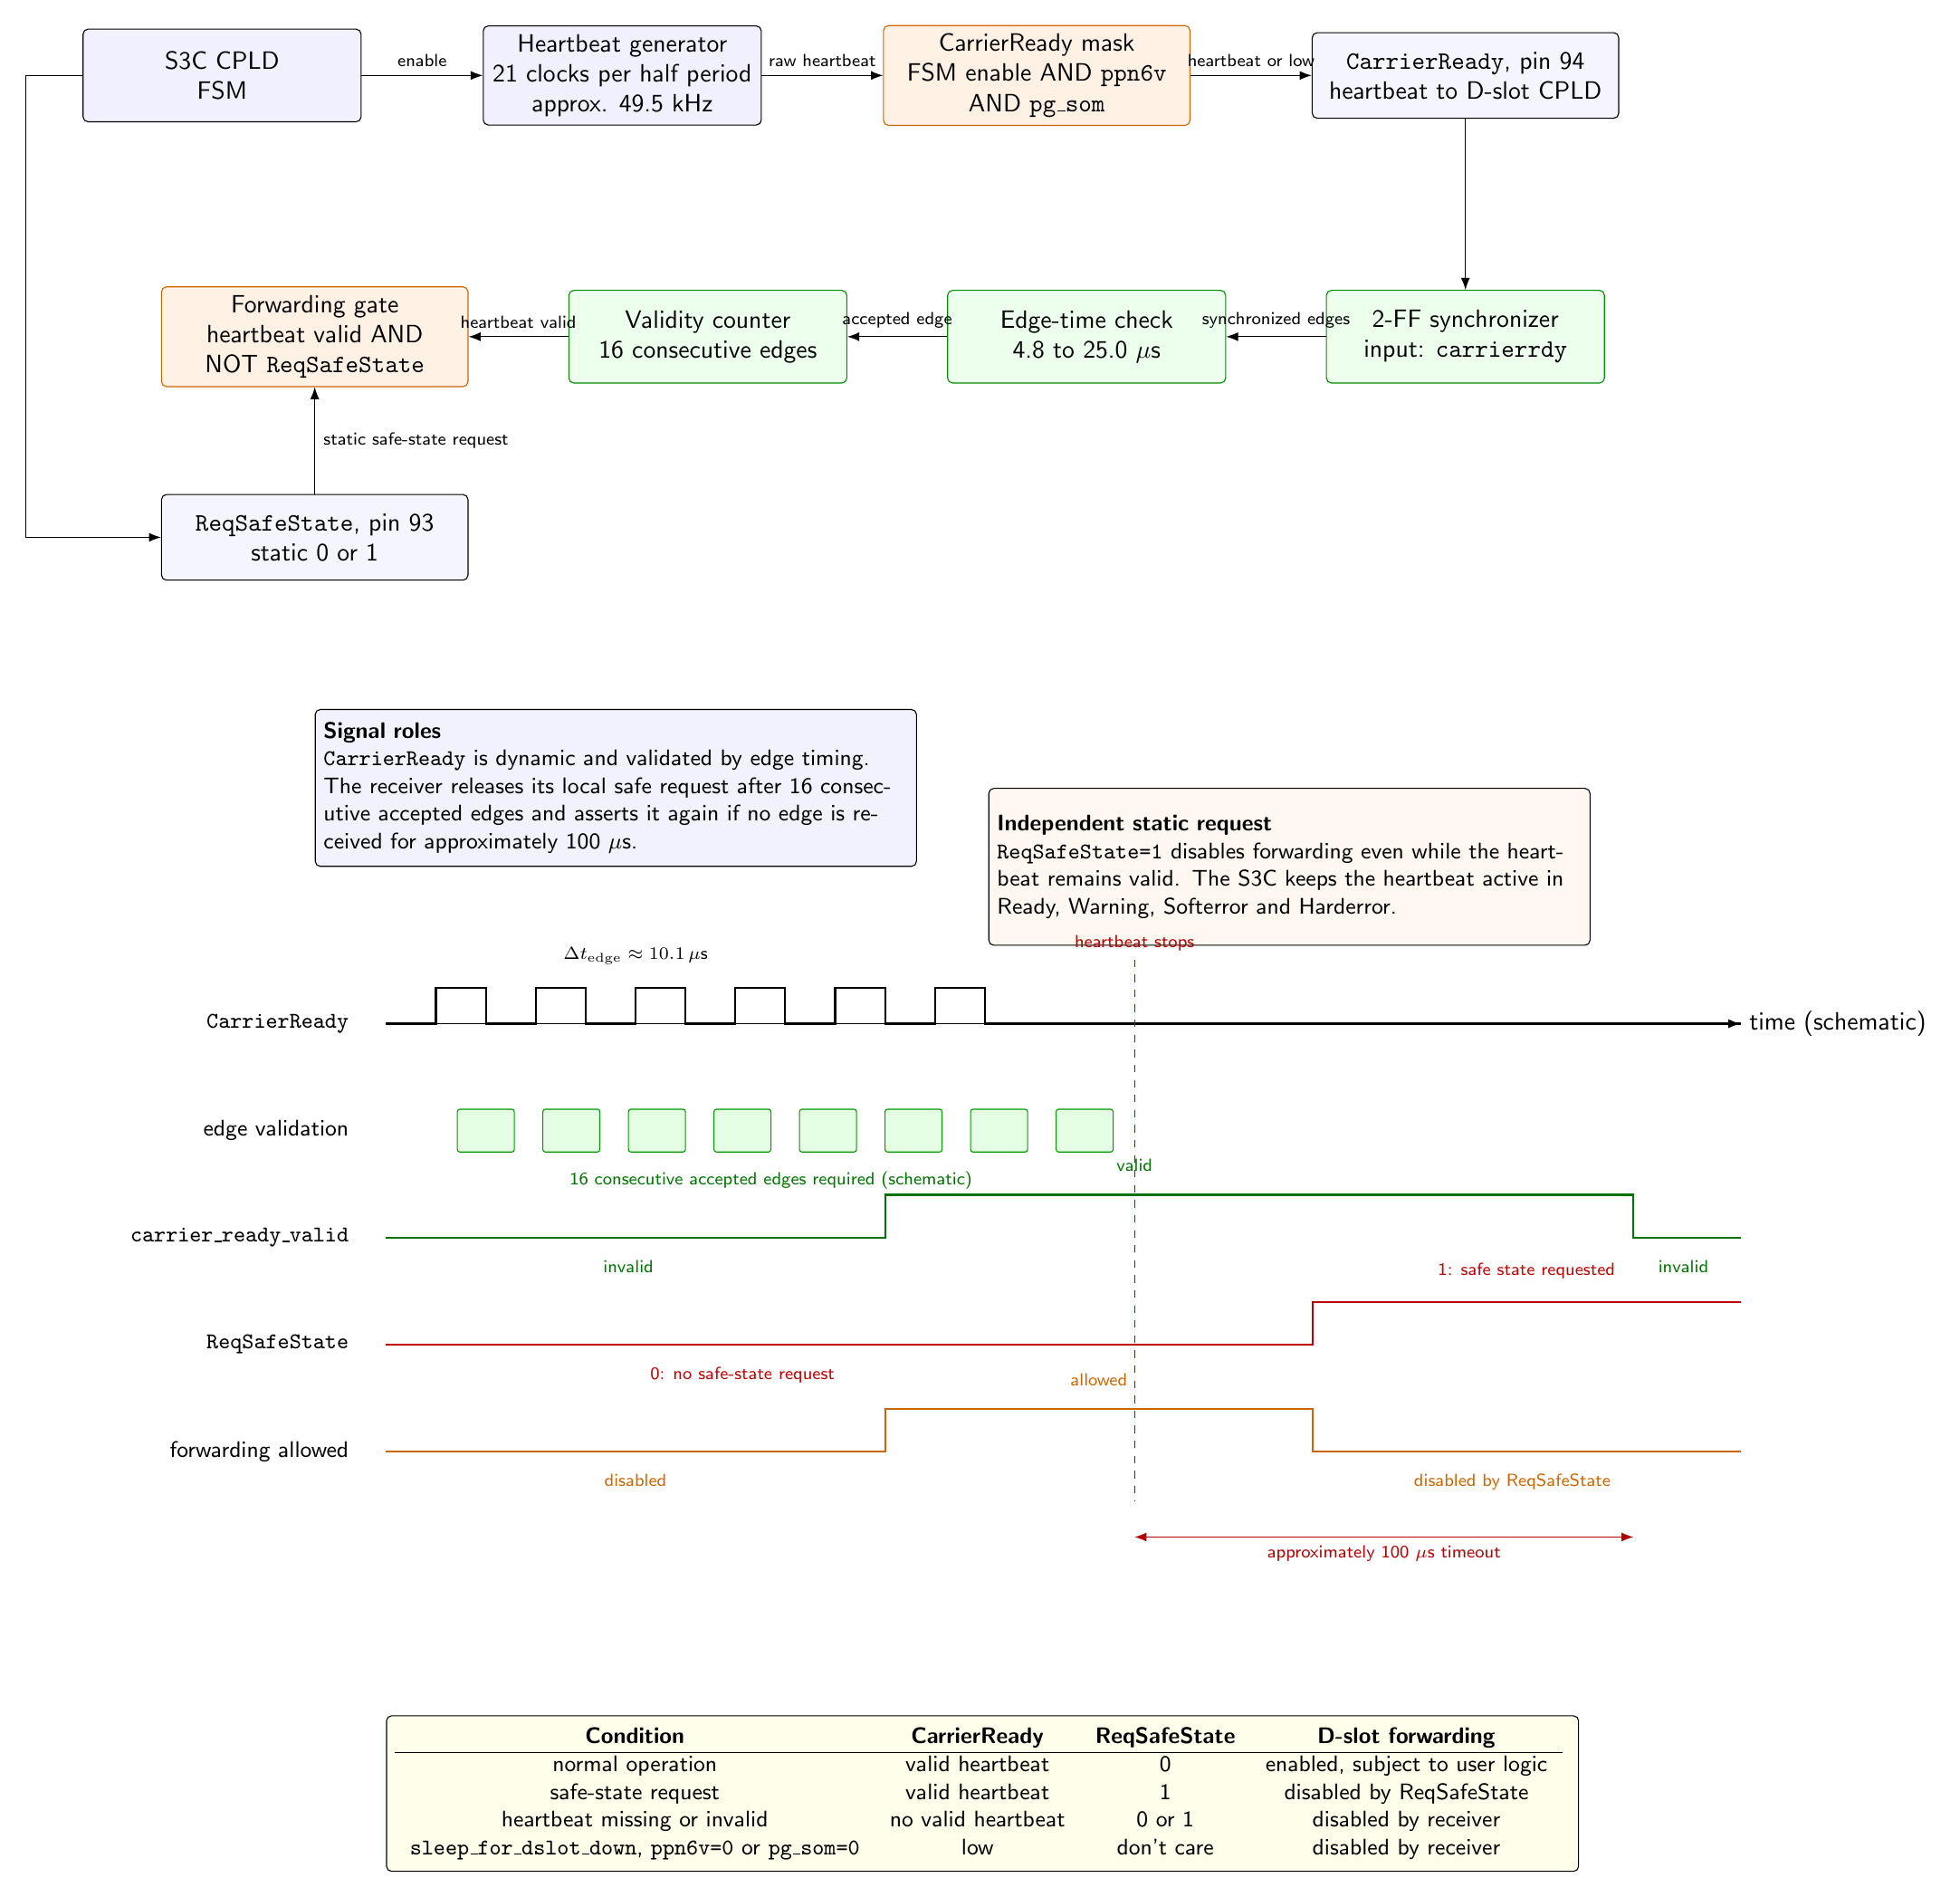
\begin{tikzpicture}[
  font=\sffamily,
  >=Latex,
  block/.style={draw, rounded corners=2pt, align=center, minimum height=13mm,
                minimum width=39mm, fill=blue!6},
  dblock/.style={draw=green!55!black, rounded corners=2pt, align=center,
                 minimum height=13mm, minimum width=39mm, fill=green!7},
  gate/.style={draw=orange!80!black, rounded corners=2pt, align=center,
               minimum height=13mm, minimum width=43mm, fill=orange!10},
  signal/.style={draw, rounded corners=2pt, align=center, minimum height=12mm,
                 minimum width=43mm, fill=blue!4},
  info/.style={draw, rounded corners=2pt, align=left, font=\sffamily\small,
               text width=82mm, minimum height=22mm},
  note/.style={font=\sffamily\small, align=center},
  tiny/.style={font=\sffamily\scriptsize, align=center},
  sig/.style={thick},
  accepted/.style={draw=green!60!black, fill=green!10, rounded corners=1pt}
]

% S3C path
\node[block] (fsm) {S3C CPLD\\FSM};
\node[block, right=17mm of fsm] (generator)
  {Heartbeat generator\\21 clocks per half period\\approx. 49.5 kHz};
\node[gate, right=17mm of generator] (mask)
  {CarrierReady mask\\FSM enable AND \texttt{ppn6v}\\AND \texttt{pg\_som}};
\node[signal, right=17mm of mask] (carrier)
  {\texttt{CarrierReady}, pin 94\\heartbeat to D-slot CPLD};

\draw[->] (fsm) -- node[above,tiny] {enable} (generator);
\draw[->] (generator) -- node[above,tiny] {raw heartbeat} (mask);
\draw[->] (mask) -- node[above,tiny] {heartbeat or low} (carrier);

% D-slot receiver path on a separate row
\node[dblock, below=24mm of carrier] (sync)
  {2-FF synchronizer\\input: \texttt{carrierrdy}};
\node[dblock, left=14mm of sync] (window)
  {Edge-time check\\4.8 to 25.0 $\mu$s};
\node[dblock, left=14mm of window] (counter)
  {Validity counter\\16 consecutive edges};
\node[gate, left=14mm of counter] (forward)
  {Forwarding gate\\heartbeat valid AND\\NOT \texttt{ReqSafeState}};

\draw[->] (carrier) -- (sync);
\draw[->] (sync) -- node[above,tiny] {synchronized edges} (window);
\draw[->] (window) -- node[above,tiny] {accepted edge} (counter);
\draw[->] (counter) -- node[above,tiny] {heartbeat valid} (forward);

% Independent static safe-state path on a third row
\node[signal, below=15mm of forward] (reqsafe)
  {\texttt{ReqSafeState}, pin 93\\static 0 or 1};
\draw[->] (fsm.west) -- ++(-8mm,0) |- (reqsafe.west);
\draw[->] (reqsafe.north) -- node[right,tiny]
  {static safe-state request} (forward.south);

\node[info, fill=blue!5, below=18mm of reqsafe, anchor=north west] (params) {
  \textbf{Signal roles}\\
  \texttt{CarrierReady} is dynamic and validated by edge timing.
  The receiver releases its local safe request after 16 consecutive accepted edges
  and asserts it again if no edge is received for approximately 100 $\mu$s.
};
\node[info, fill=orange!6, right=10mm of params, anchor=north west] (states) {
  \textbf{Independent static request}\\
  \texttt{ReqSafeState=1} disables forwarding even while the heartbeat remains valid.
  The S3C keeps the heartbeat active in Ready, Warning, Softerror and Harderror.
};

% Schematic timing diagram. Horizontal spacing is intentionally not to scale.
\coordinate (t0) at ($(params.south west)+(10mm,-22mm)$);
\draw[->] (t0) -- ++(190mm,0) node[right] {time (schematic)};
\node[note, anchor=east] at ($(t0)+(-4mm,0mm)$) {\texttt{CarrierReady}};
\node[note, anchor=east] at ($(t0)+(-4mm,-15mm)$) {edge validation};
\node[note, anchor=east] at ($(t0)+(-4mm,-30mm)$)
  {\texttt{carrier\_ready\_valid}};
\node[note, anchor=east] at ($(t0)+(-4mm,-45mm)$)
  {\texttt{ReqSafeState}};
\node[note, anchor=east] at ($(t0)+(-4mm,-60mm)$) {forwarding allowed};

% Heartbeat continues beyond validation, then stops.
\draw[sig] ($(t0)+(0,0)$)
  -- ++(7mm,0) -- ++(0,5mm) -- ++(7mm,0) -- ++(0,-5mm)
  -- ++(7mm,0) -- ++(0,5mm) -- ++(7mm,0) -- ++(0,-5mm)
  -- ++(7mm,0) -- ++(0,5mm) -- ++(7mm,0) -- ++(0,-5mm)
  -- ++(7mm,0) -- ++(0,5mm) -- ++(7mm,0) -- ++(0,-5mm)
  -- ++(7mm,0) -- ++(0,5mm) -- ++(7mm,0) -- ++(0,-5mm)
  -- ++(7mm,0) -- ++(0,5mm) -- ++(7mm,0) -- ++(0,-5mm)
  -- ++(21mm,0) -- ++(85mm,0);
\draw[dashed, red!70!black] ($(t0)+(105mm,9mm)$) -- ($(t0)+(105mm,-67mm)$);
\node[tiny, red!70!black, anchor=south] at ($(t0)+(105mm,9mm)$)
  {heartbeat stops};
\node[tiny, anchor=south] at ($(t0)+(35mm,7mm)$)
  {$\Delta t_{\mathrm{edge}}\approx10.1\,\mu$s};

% Accepted edge sequence (schematic; not every edge is drawn).
\foreach \x in {10,22,34,46,58,70,82,94} {
  \draw[accepted] ($(t0)+(\x mm,-18mm)$) rectangle ++(8mm,6mm);
}
\node[tiny, green!45!black] at ($(t0)+(54mm,-22mm)$)
  {16 consecutive accepted edges required (schematic)};

% Validity is active-high and drops after timeout.
\draw[sig, green!45!black] ($(t0)+(0,-30mm)$) -- ++(70mm,0)
  -- ++(0,6mm) -- ++(105mm,0)
  -- ++(0,-6mm) -- ++(15mm,0);
\node[tiny, green!45!black, anchor=north] at ($(t0)+(34mm,-32mm)$) {invalid};
\node[tiny, green!45!black, anchor=south] at ($(t0)+(105mm,-22mm)$) {valid};
\node[tiny, green!45!black, anchor=north] at ($(t0)+(182mm,-32mm)$) {invalid};

% ReqSafeState is independently asserted while heartbeat remains valid.
\draw[sig, red!75!black] ($(t0)+(0,-45mm)$) -- ++(130mm,0)
  -- ++(0,6mm) -- ++(60mm,0);
\node[tiny, red!75!black, anchor=north] at ($(t0)+(50mm,-47mm)$)
  {0: no safe-state request};
\node[tiny, red!75!black, anchor=south] at ($(t0)+(160mm,-37mm)$)
  {1: safe state requested};

% Final forwarding permission is active-high.
\draw[sig, orange!80!black] ($(t0)+(0,-60mm)$) -- ++(70mm,0)
  -- ++(0,6mm) -- ++(60mm,0)
  -- ++(0,-6mm) -- ++(60mm,0);
\node[tiny, orange!80!black, anchor=north] at ($(t0)+(35mm,-62mm)$) {disabled};
\node[tiny, orange!80!black, anchor=south] at ($(t0)+(100mm,-52mm)$) {allowed};
\node[tiny, orange!80!black, anchor=north] at ($(t0)+(158mm,-62mm)$)
  {disabled by ReqSafeState};

% Timeout annotation: heartbeat stop to loss of validity.
\draw[<->, red!70!black] ($(t0)+(105mm,-72mm)$)
  -- node[below,tiny] {approximately 100 $\mu$s timeout} ($(t0)+(175mm,-72mm)$);

% Truth table
\node[draw, rounded corners=2pt, fill=yellow!8, align=center,
      font=\sffamily\small, below=25mm of t0, yshift=-72mm, anchor=north west] {
\begin{tabular}{c c c c}
\textbf{Condition} & \textbf{CarrierReady}
& \textbf{ReqSafeState} & \textbf{D-slot forwarding}\\
\hline
normal operation & valid heartbeat & 0 & enabled, subject to user logic\\
safe-state request & valid heartbeat & 1 & disabled by ReqSafeState\\
heartbeat missing or invalid & no valid heartbeat & 0 or 1 & disabled by receiver\\
\texttt{sleep\_for\_dslot\_down}, \texttt{ppn6v=0} or \texttt{pg\_som=0}
& low & don't care & disabled by receiver
\end{tabular}
};

\end{tikzpicture}
\end{document}
